Stuff here about the project and aims and such.

\section{A Brief History of Golf}

The origins of the game of golf are difficult to trace, with suggestions that the game originated
in either Scotland, France, the Netherlands, China, or even going back as far as the Roman Empire.
Golf in its more modern incarnation however, is agreed to have originated in the \nth{15} century in
Scotland, where the first written records of the game are (somewhat humorously) related to
King James II of Scotland banning the game in 1457 for fear of a decrease in archery practice
in its favour.

From the \nth{18} century onwards golf began to take form fully in Scotland, with the founding
of both The Royal and Ancient Golf Club in St Andrews and The Royal Burgess Golfing Society
in Edinburgh. The oldest surviving rules of golf also date from this time and these rules have been
in a state of constant revision up to the modern day.

In the \nth{19} century the popularity of golf vastly increased, seeing larger numbers of people
knowing and playing the game, and the start of the first major tournaments. Additionally, the
game spread out to encompass much of the British empire, to the United States and eventually to
Japan, making golf into a global sport supported by a plethora of associated manufacturers, sponsors
and organisations.

In the modern day, golf is potentially one of the largest sports on earth, with golf tournaments,
golf manufacturing and related industries accounting for hundreds of billions of pounds of
economic activity. If successful on the golf tournament circuit, golf professionals can earn huge sums
in prize money. With the players themselves and their sponsors having such a vested interest in success
having a consistent and fair rule set is of paramount importance and this is dealt with jointly by 
The R\&A in most of the world and the USGA (United States Golf Association) 
in the Americas.

\section{A Slightly Larger History of the Golf Ball}

Golf ball technology has advanced greatly since the advent of the game. Initially, hard wooden
balls were used for playing, however these were soon replaced with “featherie” balls which are
leather pouches stuffed with feathers and then painted white.

The next major innovation in the design of golf balls came in 1848, when the gutta-percha
ball was invented. This is the first ball to use a rubbery substance as continues to this day,
and was easier to make into a proper sphere, unlike the previous types of ball. It was around
this time that it was discovered that abrasions to the surface of the ball would improve the
aerodynamic properties of the ball, making it easier to control the flight of the ball and increasing
the distance at which the game could be played. This would start a series of innovations that
would lead to today’s dimpled balls, which we will discuss later.

\begin{figure}[h]
\centering
\begin{subfigure}[b]{0.4\textwidth}
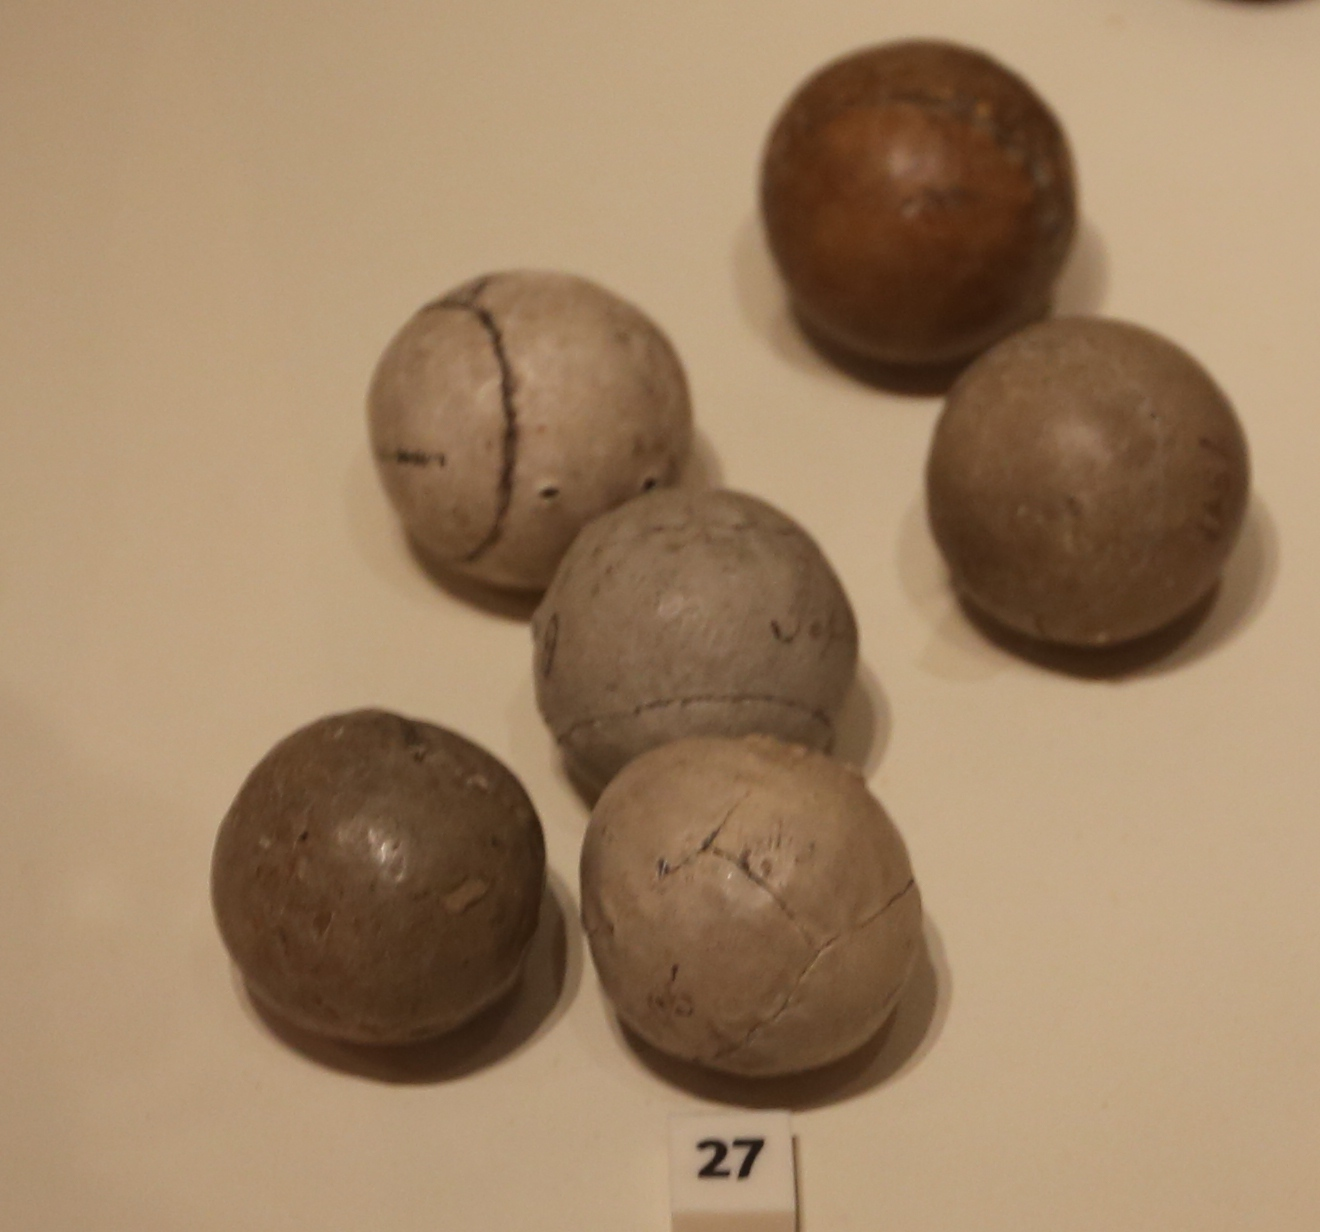
\includegraphics[scale=0.16]{../images/featherie.jpg}
\caption{``Featherie'' balls}
\label{im:featherie}
\end{subfigure}
\quad \quad \quad \quad
\begin{subfigure}[b]{0.4\textwidth}
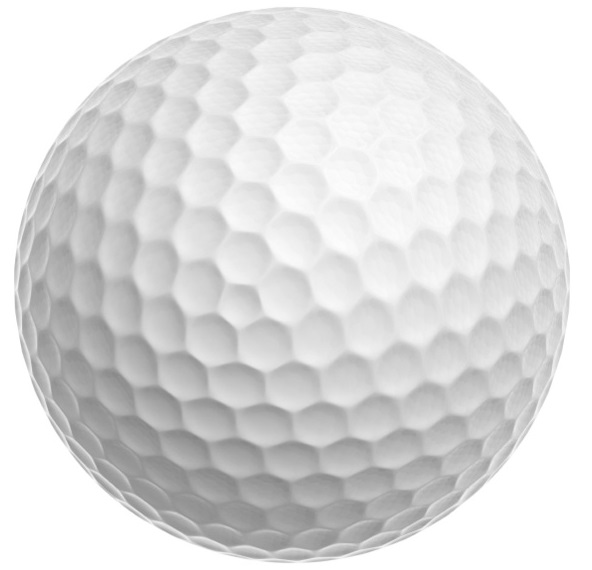
\includegraphics[scale=0.48]{../images/golf-itemno-12.jpg}
\caption{A modern style ball}
\label{im:pv1}
\end{subfigure}
\caption[Images of golf balls]{In \ref{im:featherie} are ``Featherie'' golf balls, taken from 
\url{https://en.wikipedia.org/wiki/File:Featherie_golf_ball.JPG}, 
and in \ref{im:pv1} is a modern style ball.}
\end{figure}

After this the golf ball once again changed form with the advent of using wrapped rubber
thread to help the ball to bounce better. This was coupled with the first usage of a plastic 
covering, in order to protect the rubber inside the ball on impact with the
club. This cover also persists to this day, although the inside of the ball has seen significant
development.

The modern golf ball has changed significantly from old designs. The interior of the ball is
now usually a 3 piece rubber composite, with different properties in each rubber to maximize
the controllability of the ball during play. The exterior is a polyurethane cover (normally white
but some are in other colours) with usually between 300 to 400 dimples (though these can go as 
low as 200 dimples, and beyond 600 in some cases). The properties of the ball are stipulated to be
within certain ranges, as set by The R\&A and USGA in the rules of golf. The weight of a ball must
not be greater than 45.93g, the diameter no less than 42.67mm and the ball must be spherically symmetric.

\section{Aims of the Project}

The aim of this project is to obtain a model for how golf balls fly based on an understanding of the
fluid mechanics governing the flight of a golf ball. Using this knowledge, we then wish to obtain a
simple physical model which describes most, if not all, of the behaviour as the ball flies.

Given this model we then wish to categorise individual balls based on measurements of their flight, and
use this categorisation to predict trajectories for the ball based on different initial conditions.
Finally, using this model, we will attempt to use a limited set of flight data (between 20 and 30 m)
to predict the full flight for the ball.